\documentclass[a4paper,12pt]{article}
\RequirePackage[a4paper,top=1cm,bottom=2cm,left=1.8cm,right=1.8cm]{geometry}
\date{}
%\nofiles

\usepackage{graphicx}


\begin{document}

\title{Pin alignment using multiple top camera images}
\maketitle

%%%%%%%%%%%%%%%%%%%%%%%%%%%%%%%%%%%%%%%%%%%%%%%%%%%%%%%%%%%%%%%%%%%%%%%%%%%%%%%%%%%%%%%%%%%%%%%%%%%%%%%%%%%%%%%%%%%%%%
%%%%%%%%%%%%%%%%%%%%%%%%%%%%%%%%%%%%%%%%%%%%%%%%%%%%%%%%%%%%%%%%%%%%%%%%%%%%%%%%%%%%%%%%%%%%%%%%%%%%%%%%%%%%%%%%%%%%%%
%%%%%%%%%%%%%%%%%%%%%%%%%%%%%%%%%%%%%%%%%%%%%%%%%%%%%%%%%%%%%%%%%%%%%%%%%%%%%%%%%%%%%%%%%%%%%%%%%%%%%%%%%%%%%%%%%%%%%%


\section{Introduction}

To align the pin on the center of the diffractometer you need to move the diffractometer to various angles and adjust the $x$, $y$ and $z$ positions so that the rotation occurs around one fixed point. Instead of making iterative changes it is possible to collect multiple images of the pin with a fixed, unknown offset from the center of rotation. Using the coordinates of the pin in each image and doing post-processing fitting you can determine the motor positions needed to get the pin to the center of the diffractometer. Whilst collecting the images this method does not need user intervention and also the fit parameters and their uncerntanties give the level of confidence in the pin alignment. 




First the cryostat moves to series of different positions and take an image of the pin at each position. Once this is finished the location of the pin in each image is identified and then a vector is fitted which relates the origin of the motor coordinates to the center of rotation of the diffractometer. Figure \ref{images_top} shows images in the $xy$ plane of the pin with $\theta = +90$ and $-90$ and with $\chi = 86$, $90$ and $94$. The pin rotates around the center of the diffractometer and in this case the $y$ motor position has been offset to show the circle that the pin rotates around. 

\begin{figure}[tbh]
	\centering
	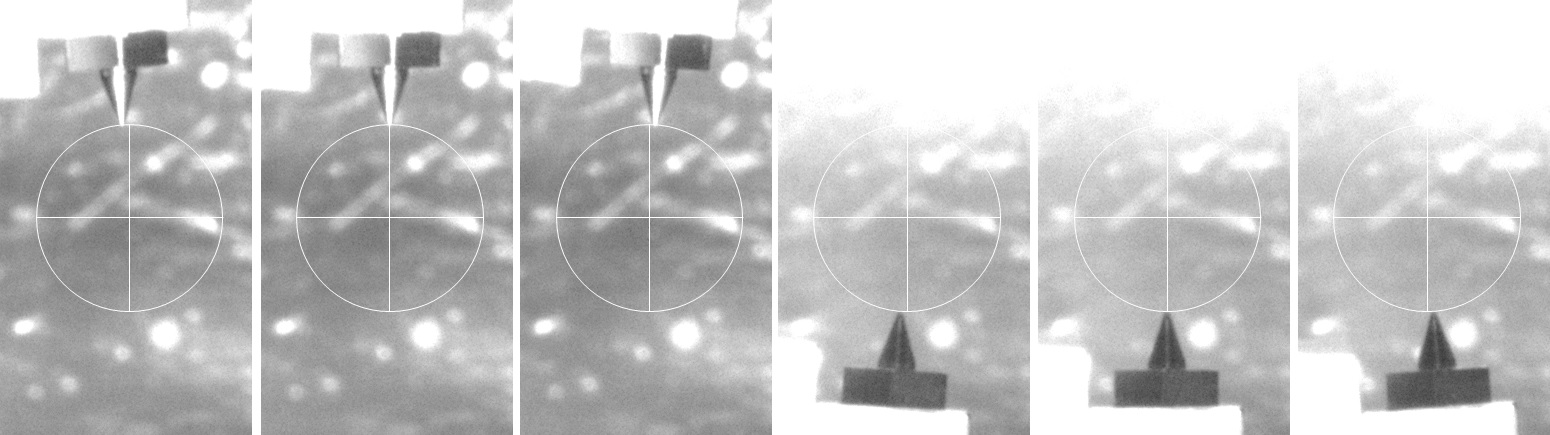
\includegraphics[width=17cm]{graphics/images_top.jpg}
	\caption{Images in the $xy$ plane of the pin with $\theta = +90$ and $-90$ and with $\chi = 86$, $90$ and $94$.}
	\label{images_top}
\end{figure}

The vector from the fitting is then used to adjust the cryostat motor calibrations. The fitting also provides the calibration of the pixel size of the camera and the pixel coordinates of the center of the diffractometer on the camera.


Similar images in the $yz$ plane in figure \ref{images_side} also show the position of the pin. However, due to the cabling the images are not as clear and the alignment based on these images is not as accurate.

\begin{figure}[tbh]
	\centering
	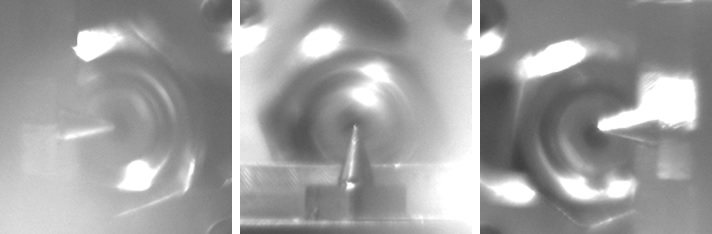
\includegraphics[width=10cm]{graphics/images_side.jpg}
	\caption{Images in the $yz$ plane of the pin with $\theta = +90$, $0$ and $-90$.}
	\label{images_side}
\end{figure}




%%%%%%%%%%%%%%%%%%%%%%%%%%%%%%%%%%%%%%%%%%%%%%%%%%%%%%%%%%%%%%%%%%%%%%%%%%%%%%%%%%%%%%%%%%%%%%%%%%%%%%%%%%%%%%%%%%%%%%
%%%%%%%%%%%%%%%%%%%%%%%%%%%%%%%%%%%%%%%%%%%%%%%%%%%%%%%%%%%%%%%%%%%%%%%%%%%%%%%%%%%%%%%%%%%%%%%%%%%%%%%%%%%%%%%%%%%%%%
%%%%%%%%%%%%%%%%%%%%%%%%%%%%%%%%%%%%%%%%%%%%%%%%%%%%%%%%%%%%%%%%%%%%%%%%%%%%%%%%%%%%%%%%%%%%%%%%%%%%%%%%%%%%%%%%%%%%%%



\section{Alignment tests}

The alignment process was repeated multiple times. Each time takes approximately 20 minuets to capture the images. The variation in the fit parameters for $x$, $y$ and $z$ are shown in figure \ref{different_image_variation}.


\begin{figure}[tbh]
	\centering
	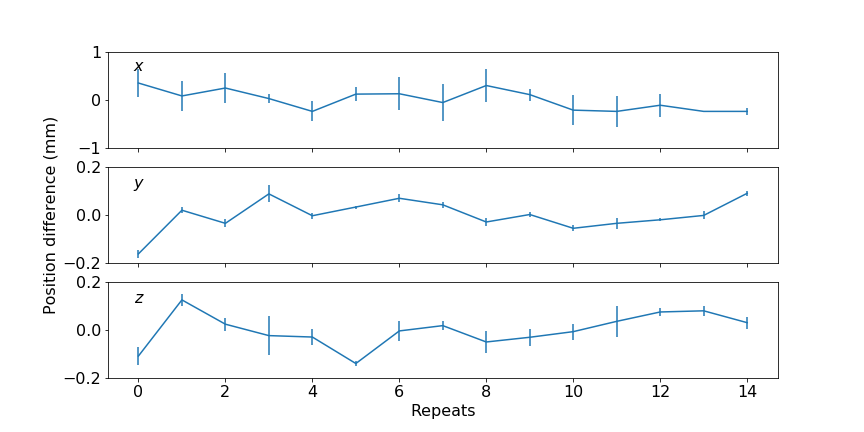
\includegraphics[width=17cm]{graphics/different_image_variation.png}
	\caption{Differences in $x$, $y$ and $z$ fit parameters repeating the image capture and fitting multiple times.}
	\label{different_image_variation}
\end{figure}

The error bars are the errors given out from the fits in each alignment. The standard deviation between the different points is:

$\delta x$ = 203~$\mu m$, $\delta y$ = 62~$\mu m$ and $\delta z$ = 67~$\mu m$.

	



%%%%%%%%%%%%%%%%%%%%%%%%%%%%%%%%%%%%%%%%%%%%%%%%%%%%%%%%%%%%%%%%%%%%%%%%%%%%%%%%%%%%%%%%%%%%%%%%%%%%%%%%%%%%%%%%%%%%%%
%%%%%%%%%%%%%%%%%%%%%%%%%%%%%%%%%%%%%%%%%%%%%%%%%%%%%%%%%%%%%%%%%%%%%%%%%%%%%%%%%%%%%%%%%%%%%%%%%%%%%%%%%%%%%%%%%%%%%%
%%%%%%%%%%%%%%%%%%%%%%%%%%%%%%%%%%%%%%%%%%%%%%%%%%%%%%%%%%%%%%%%%%%%%%%%%%%%%%%%%%%%%%%%%%%%%%%%%%%%%%%%%%%%%%%%%%%%%%



\section{Repeat alignment with same images}

Using the same images and repeating the process several times gives a measure of how good this alignment technique is. This time the variation in the fit parameters for $x$, $y$ and $z$ are shown in figure \ref{same_image_variation}.

\begin{figure}[tbh]
	\centering
	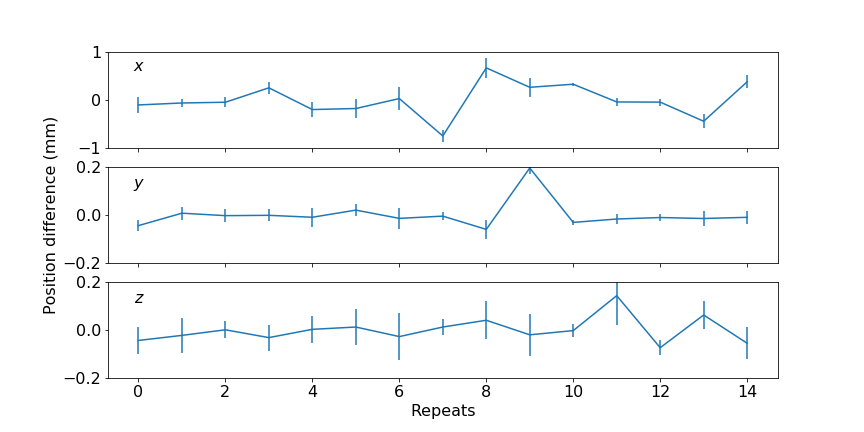
\includegraphics[width=17cm]{graphics/same_image_variation.png}
	\caption{Differences in $x$, $y$ and $z$ fit parameters where the analysis was repeated on the same set of images multiple times.}
	\label{same_image_variation}
\end{figure}


The standard deviation between the different points is:

$\delta x$ = 335~$\mu m$, $\delta y$ = 56~$\mu m$ and $\delta z$ = 51~$\mu m$.


For $y$ and $z$, there is less variation between the repeats of the alignment using the same images. However, it isn't significantly less. This implies that the motor movements positioning the pin are quite accurate and that the inaccuracies in the alignment originate from the method of using the camera. For $x$ the errors from repeating the alignment with the same images is actually larger than for the repeats with different images.

This alignment method is good for getting the pin within $340~\mu m$ in $x$ and to within $70~\mu m$ in $y$ and $z$.

%%%%%%%%%%%%%%%%%%%%%%%%%%%%%%%%%%%%%%%%%%%%%%%%%%%%%%%%%%%%%%%%%%%%%%%%%%%%%%%%%%%%%%%%%%%%%%%%%%%%%%%%%%%%%%%%%%%%%%
%%%%%%%%%%%%%%%%%%%%%%%%%%%%%%%%%%%%%%%%%%%%%%%%%%%%%%%%%%%%%%%%%%%%%%%%%%%%%%%%%%%%%%%%%%%%%%%%%%%%%%%%%%%%%%%%%%%%%%
%%%%%%%%%%%%%%%%%%%%%%%%%%%%%%%%%%%%%%%%%%%%%%%%%%%%%%%%%%%%%%%%%%%%%%%%%%%%%%%%%%%%%%%%%%%%%%%%%%%%%%%%%%%%%%%%%%%%%%


\subsection{Future improvements}

To further improve the alignment of the center of the diffractometer the pin could be made smaller or the zoom on the camera could be increased. The limiting factor is how well we can measure the alignment rather than the alignment itself.

Having a permanent, non-movable light source would make the images more similar and may allow for using image recognition to detect the pin position. This may remove the aspect of human error from identifying the pin in the captured images.


%%%%%%%%%%%%%%%%%%%%%%%%%%%%%%%%%%%%%%%%%%%%%%%%%%%%%%%%%%%%%%%%%%%%%%%%%%%%%%%%%%%%%%%%%%%%%%%%%%%%%%%%%%%%%%%%%%%%%%
%%%%%%%%%%%%%%%%%%%%%%%%%%%%%%%%%%%%%%%%%%%%%%%%%%%%%%%%%%%%%%%%%%%%%%%%%%%%%%%%%%%%%%%%%%%%%%%%%%%%%%%%%%%%%%%%%%%%%%
%%%%%%%%%%%%%%%%%%%%%%%%%%%%%%%%%%%%%%%%%%%%%%%%%%%%%%%%%%%%%%%%%%%%%%%%%%%%%%%%%%%%%%%%%%%%%%%%%%%%%%%%%%%%%%%%%%%%%%




\subsection{$sx$ movement}

As well as being used to find the center of the diffractometer, the images provide a calibration of the camera pixels to the movement on the sample holder. Figure \ref{sx_movement} shows how the $x$ and $y$ pixel coordinates change as the cryostat is moved in the $x$ direction.

\begin{figure}[tbh]
	\centering
	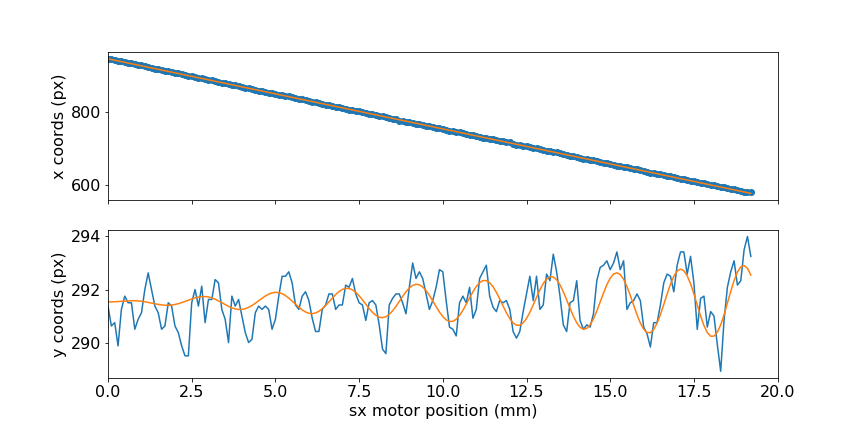
\includegraphics[width=17cm]{graphics/sx_movement.png}
	\caption{Position of the pin on the camera as the cryostate is moved in $sx$.}
	\label{sx_movement}
\end{figure}

The top images shows that the $x$ motion of the cryostat moves the pin in the $x$ coordinate of the camera. The gradient provides a calibration of 18.964 $\pm$ 0.009~$px/mm$.

The bottom image shows that there is some coupling between the $x$ and $y$ motion of the cryostat. This appears to make a spiral pattern as $x$ is moved where the peak to peak motion in $y$ gets up to 3~$px$ which is 153~$\mu m$.




%%%%%%%%%%%%%%%%%%%%%%%%%%%%%%%%%%%%%%%%%%%%%%%%%%%%%%%%%%%%%%%%%%%%%%%%%%%%%%%%%%%%%%%%%%%%%%%%%%%%%%%%%%%%%%%%%%%%%%
%%%%%%%%%%%%%%%%%%%%%%%%%%%%%%%%%%%%%%%%%%%%%%%%%%%%%%%%%%%%%%%%%%%%%%%%%%%%%%%%%%%%%%%%%%%%%%%%%%%%%%%%%%%%%%%%%%%%%%
%%%%%%%%%%%%%%%%%%%%%%%%%%%%%%%%%%%%%%%%%%%%%%%%%%%%%%%%%%%%%%%%%%%%%%%%%%%%%%%%%%%%%%%%%%%%%%%%%%%%%%%%%%%%%%%%%%%%%%





\end{document}
